\documentclass[11pt,fleqn]{article}
%\usepackage{CJK}
\usepackage{latexsym}
\usepackage{color}
\usepackage{graphicx, float}\usepackage{graphicx}
%\usepackage{algorithmicx}
\usepackage{algorithm}
\usepackage{algpseudocode}
%\usepackage[colorlinks]{hyperref}
\usepackage[toc,page]{appendix}
\usepackage{bm}
\setlength{\oddsidemargin}{-0.0in}
\setlength{\evensidemargin}{-0.0in} \setlength{\textwidth}{6.0in}
\setlength{\textheight}{9.0in} \setlength{\topmargin}{-0.2in}

%\setlength{\leftmargin}{0.7in}
\usepackage{amssymb, graphicx, amsmath}  %  fancyheadings,
\usepackage{setspace}
\newcommand\qed{\qquad $\square$}
\newcommand{\nn}{\nonumber}

\def \[{\begin{equation}}
\def \]{\end{equation}}
\def\proof{{\bf Proof:\quad}}
\def \endzm {\quad $\Box$}
\def\dist{\hbox{dist}}


\newcommand{\R}{\mathbb{R}}
%\newtheorem{yinli}{����}[section]
\newcommand{\D}{\displaystyle}
\newcommand{\T}{\textstyle}
\newcommand{\SC}{\scriptstyle}
\newcommand{\FT}{\footnotesize}

% https://tex.stackexchange.com/questions/88414/how-can-i-create-a-question-answer-format-for-reports
\usepackage{enumitem}
\newenvironment{QandA}{\begin{enumerate}\bfseries}
                      {\end{enumerate}}
\newenvironment{answered}{\par\normalfont}{}
\usepackage{lipsum}

\usepackage{hyperref}
\newcommand\fnurl[2]{%
  \href{#2}{#1}\footnote{\url{#2}}%
}

%\newtheorem{theorem}{Theorem}[section]
%\renewcommand{\thetheorem}{\arabic{section}.\arabic{theorem}}
\newtheorem{definition}{Definition}
\renewcommand{\thedefinition}{\arabic{section}.\arabic{definition}}
\newtheorem{lemma}{Lemma}[section]
\renewcommand{\thelemma}{\arabic{section}.\arabic{lemma}}
\newtheorem{remark}{Remark}
\renewcommand{\theremark}{\arabic{section}.\arabic{remark}}
\newtheorem{proposition}{Proposition}[section]
\renewcommand{\theproposition}{\arabic{section}.\arabic{proposition}}
\newtheorem{corollary}{Corollary }[section]
\renewcommand{\thecorollary}{\arabic{section}.\arabic{corollary}}
\renewcommand{\theequation}{\arabic{section}.\arabic{equation}}
\renewcommand{\baselinestretch}{1.35}
\newtheorem{exam}{Example}[section]
\renewcommand{\theexam}{\arabic{section}.\arabic{exam}}
\newtheorem{theo}{Theorem}[section]
\renewcommand{\thetheo}{\arabic{section}.\arabic{theo}}
\begin{document}
%\begin{CJK*}{GBK}{song}

\begin{center}

{\LARGE \bf CS380D Distributed Systems Review Questions }\\

\vskip 25pt
 {Zeyuan Hu, iamzeyuanhu@utexas.edu }\\
\vskip 5pt
{\small EID:zh4378 Spring 2018 }

\end{center}

\section{Jan 19 Review Questions}
\begin{QandA}
   \item How do the 8 fallacies of distributed systems differ between designing a system over the world wide web (say between India and the US) and between servers inside a single datacenter? 
         \begin{answered}
         \begin{enumerate}
          \item The network is reliable. The network for a system that spans globablly may be highly likely unreliable. However, for a system
          resides only in a single datacenter. We can think the network is reliable. However, there are still chances for network outage even
          in a single datacenter.
          \item Latency is zero. The latency for a global system is necessarily non-zero and large. However, for servers in a single datacenter, we can assume that the latency is very small but we still cannot assume that the latency is zero.
          \item Bandwidth is infinite. No matter which scenarios, the bandwidth is limited.
          \item The network is secure. For servers within a single datacenter, if we have built a good firewall to isolate the network inside the
          datacenter from outside, we are likely to have a secure network. However, for a system that relies on a global network, we need to put
          much more effort to ensure the security of the network.
          \item Topology doesn't change. We can assume this one for servers in a single network. However, for a system that utilizes multiple datacenters, the topology may change over the time because we may switch to other datacenters during the time.
          \item There is one administrator. In either scenarios, we cannot assume we have one administrator. This is especially true for a global
          sytem that needs to provide a 24x7 service.
          \item Transport cost is zero. Similar to the latency, we cannot assume the transport cost is zero in either cases.
          \item The network is homogeneous. For servers in a single datacenter, we can assume this one holds. However, for a global system, this
          assumption can never be true because the network infrastructure is necessarily different from country to country.
         \end{enumerate}
         \end{answered}

   \item What would you expect to be different between Tandem's breakdown of outage reasons and the breakdown of outage reasons for a modern service, say Amazon EC2?
         \begin{answered}
         I think the administration outages still are the major source of the outage for both Tandem and a modern service given that 
         the notable outages from last year (\fnurl{GitLab}{https://about.gitlab.com/2017/02/10/postmortem-of-database-outage-of-january-31/} and \fnurl{AWS}{https://aws.amazon.com/message/41926/}) are due to the human errors. In addition, the software outage may also take the second
         place for the outage reasons given the complexity of the system has increased. However, I would expect that the outage reasons due to the
         hardware and environment may no longer hold for a modern service nowadays. The stability of hardware has increased since Tandem's paper
         and for a large scare sevice like Amazon EC2, people use multiple datacenters to provide redundancy instead of multiple servers reside in
         the same datacenter. Providing service backup using multiple datacenters across different locations make the outage due to power, communications, and facilities very unlikely.
         \end{answered}
\end{QandA}


\section{Jan 26 Review Questions}
\begin{QandA}
   \item Jeff Dean's talk mentions several patterns in distributed systems (Single Master, Many Workers; Canary Requests; ...). Describe how some of these could be applied in a current system not described in the slides.
         \begin{answered}
         Amazon EC2 system adopts ``Elastic Systems" design pattern described in the talk. A user can rent their own server(s) on the Amazon EC2. However, it is hard for user to forsee the exact peak load for his usage.
         It is expensive to rent multiple servers in the anticipation of high workload. On the other hand, the current server instances may suffer from the sudden jump in the workload, which can only be handled by renting
         additional servers. To handle this type of user's needs, Amazon EC2 system is designed to have the elastic capability to handle the workload: Amazon EC2 can automatically shrink capacity when there is not much workload and grow capacity as the workload grows. In addition, Amazon EC2 as a cloud platform can have huge amount of users' service requests. It is unfeasible to have one single machine to handle the requests from the beginning to the end. Thus, ``Tree distribution of Requests" and ``Multiple Smaller Units per Machine" design patterns can be helpful here. We restrict the amount of requests can be handled by each machine (i.e., 10-100 requests/machine) and we distribute the requests (e.g., 
         create 100 instances) to 50 leaf machines and with each leaf machine only needs to perform small amount of tasks (e.g., create two instances) . Those 50 leaf machines can connect to another tree sturcture parents and root machines to collect the status of tasks progress requested by the user.
         \end{answered}

   \item Provide an example of modern day events that are related by the happens-before relationship and an example of events that are concurrent. What are the possible relationships of the logical clock times for the events?
         \begin{answered}
		 The preference ranking on goods by a consumer. A consumer prefers $A$ over $B$ is denoted as $A \succ B$. This is similar to the "happen-before" relationship in the sense that consumer's more favorable object (i.e., $A$)
		 always comes before the less favorable object (i.e., $B$). "Concurrent" concept is also perserved in the preference ranking in the sense that if a consumer is indifferent between two goods $A$ and $B$, we can denote
		 them as $A \sim B$. In other words, if a consumer cannot tell if he perfers $A$ over $B$ or perfers $B$ over $A$, we say he is indifferent between two goods. Mathematically, $A \sim B$ when $A \nsucc B$ and $A \nprec B$,
		 which mimics concurrent definition exactly. The "logical clock times" for preference ranking is utility function where we assign numbers to each good based on the consumer's preference ranking.
		 We have $U(A) > U(B)$ if and only if $A \succ B$. In words, if the utility function value of $A$
		 is greater than $B$, we know that the consumer prefers $A$ over $B$. Reverse statement also holds. If two objects' utility function values are equal to each other (i.e., $U(A) = U(B)$), we know that the consumer
		 is indifferent between two goods (i.e., $A \sim B$).
         \end{answered}
\end{QandA}

\subsection{Feedback}

While $C(A) = C(B)$ would imply that events are concurrent, the events being concurrent doesn't actually imply $C(A) = C(B)$. 
For concurrent events $A$ and $B$, any relationship between $C(A)$ and $C(B)$ is valid. The similarity to a utility function would hold better for vector clocks, where the happens-before relationship can be inferred from the clock times.
\section{Feb 02 Review Questions}
\begin{QandA}
   \item The state machine approach paper describes implementing stability using several different clock methods. What properties does a clock need to provide so that it can be used to implement stability?
         \begin{answered}
 		 The clock should be able to assign the unique identifier to each request whose issuance corresponds to an an event. In addition, the clock should ensure the total ordering on the unique identifiers. In other words, the clock has to satisfy: 1) clock value $\hat{T_p}$ incremented after each event at process $p$ 2) Upon receipt of a message with timestamp $\tau$, process resets the clock value $\hat{T_p}$ to 
 		 $\max(\hat{T_p}, \tau) + 1$.
         \end{answered}

   \item For linearizability, sequential consistency, and eventual consistency, describe an application (real or imagined) that could reasonably use that consistency model.
         \begin{answered}
		 \begin{itemize}
		 \item linearizability example: transactions on RDBMS enforces linearizability in the sense that the read/write operations on a table in RDBMS have to be "atomic". Once a tuple is modified and commited,
		 the changes to the tuple become visible to the following read immediately. A real life example is that when I deposit the money into an 
		 account, I want to see the the money reflect the latest deposit immediately in my bank account.
		 \item sequential consistency example: isolation requirement for RDBMS. When two transactions that are modifying the same table, each operation
		 within the transactions are executed in the order they are issued. However, the operations from two transactions may be interleaved (i.e., under "Read uncommitted" isolation level). Another
		 example is one person $A$ issues "unfriend", "post" operations and the other person $B$ issues "scroll the facebook page". The operation
		 order from these two people are kept: "post" never goes before "unfriend" but operations may interleave: "unfriend", "scroll the facebook
		 page", "post" instead of doing $A$'s operation first ("unfriend", "post") and then $B$'s.
		 \item eventual consistency example: high available key-value store like Dynamo. The order status display service may not see the user's
		 update on the shopping cart but eventually those updates can be seen by every services. Another example is when you like a post, the 
		 other people who can see the post may not see your ``like" immediately in their facebook page but eventually, they will see your ``like" on the post.
		 \end{itemize}
         \end{answered}
         
   \item What's one benefit of using invalidations instead of leases? What's one benefit of using leases over invalidations?
         \begin{answered}
         One benefit of using leases over invalidations can be seen from the following example: suppose we use the eventual consistency model 
         and a write is waiting on invalidations. 
  		 Invalidation has negative impact to the system performance because the user cannot use the cache due to the invalidation but it is ok for client reads the old value because of eventual consistency. However, for the lease, if the cache is hold by the lease holder and still within the lease term, user can still read the data from the cache. This scenario also indicates the benefit of the invalidations over leases in the sense that the user may not get the latest updated value since they can read
       	the old value from the lease-holder-protected cache directly. Thus, for the linearizability consistency model, we cannot use the leases because the write may not be approved by the leaseholder and there might be a read that happens immediately after reading
       	from the out-dated cache. This violates the linearizability, which guarantees that reads always reflect the latest write. 
       	Thus, there will be a delay in write, which hinders the system performance. However, for
       	eventual consistency model, leases is more favorable than invalidations.
         \end{answered}
\end{QandA}
\section{Feb 09 Review Questions}
\begin{QandA}
   \item What are differences between strong leases and weak leases and the guarantees they provide?
         \begin{answered}
		 One difference between strong leases and weak leases is that strong leases do not allow the write while the lease held by the cache
		 hasn't expired or the leaseholder hasn't approved the write. If one object is covered by multiple strong leases, the write can happen
		 if all the leaseholders approve the write or all the leases covered that object has expired. This mechanism guarantees that there
		 will be no conflict of write to the object in cache. However, that's not ture for the weak lease. Weak leases allow the writes and reads
		 simultaneously. Same object can be owned by several weak leases with different expiration time. This implies that some leases
		 that are expired allow the writes while other non-expired leases allow the read only. Thus, we may get the conflict on the object in cache.
		 In the write-back cache, the conflict is resolved on the server side. In addition, for the weak leases,
		 the server doesn't need to keep track of the leases granted but that's not true for strong leases. Lastly, strong leases guarantess a strict
		 consistency while the weak leases have a weak consistency. As the consequence, weak lease has better performance than the strong lease
		 as we don't need to queue the writes say in the write-through for the weak lease.
         \end{answered}

   \item Use the types of anomalies allowed to per-object sequential consistency and read-after-write consistency to compare the two consistency models. Is one stronger? If so, which one?
         \begin{answered}
		 For anomalies in vetrices, both per-object sequential consistency and read-after-write consistency have stale read anomalies.
		 In addition, read-after-write consistency also has total order anomalies whereas the per-object sequential consistency doesn't. 
		 If we take a look at the actual statistics, per-object sequential consistency contains 607 total anomalise including 378 stale read
		 anomalies and 229 total order anomalies. Read-after-write consistency contains only total order anomalies. Since there is overlap between
		 read-after-write consistency anomalies and per-object sequential consistency anomalies but one of them is not the subset of the other.
		 Thus, we cannot determine which consistency model is stronger. The above text is illustrated in the Figure \ref{0209-02} as well.
		 \begin{figure}
		 \centering
		 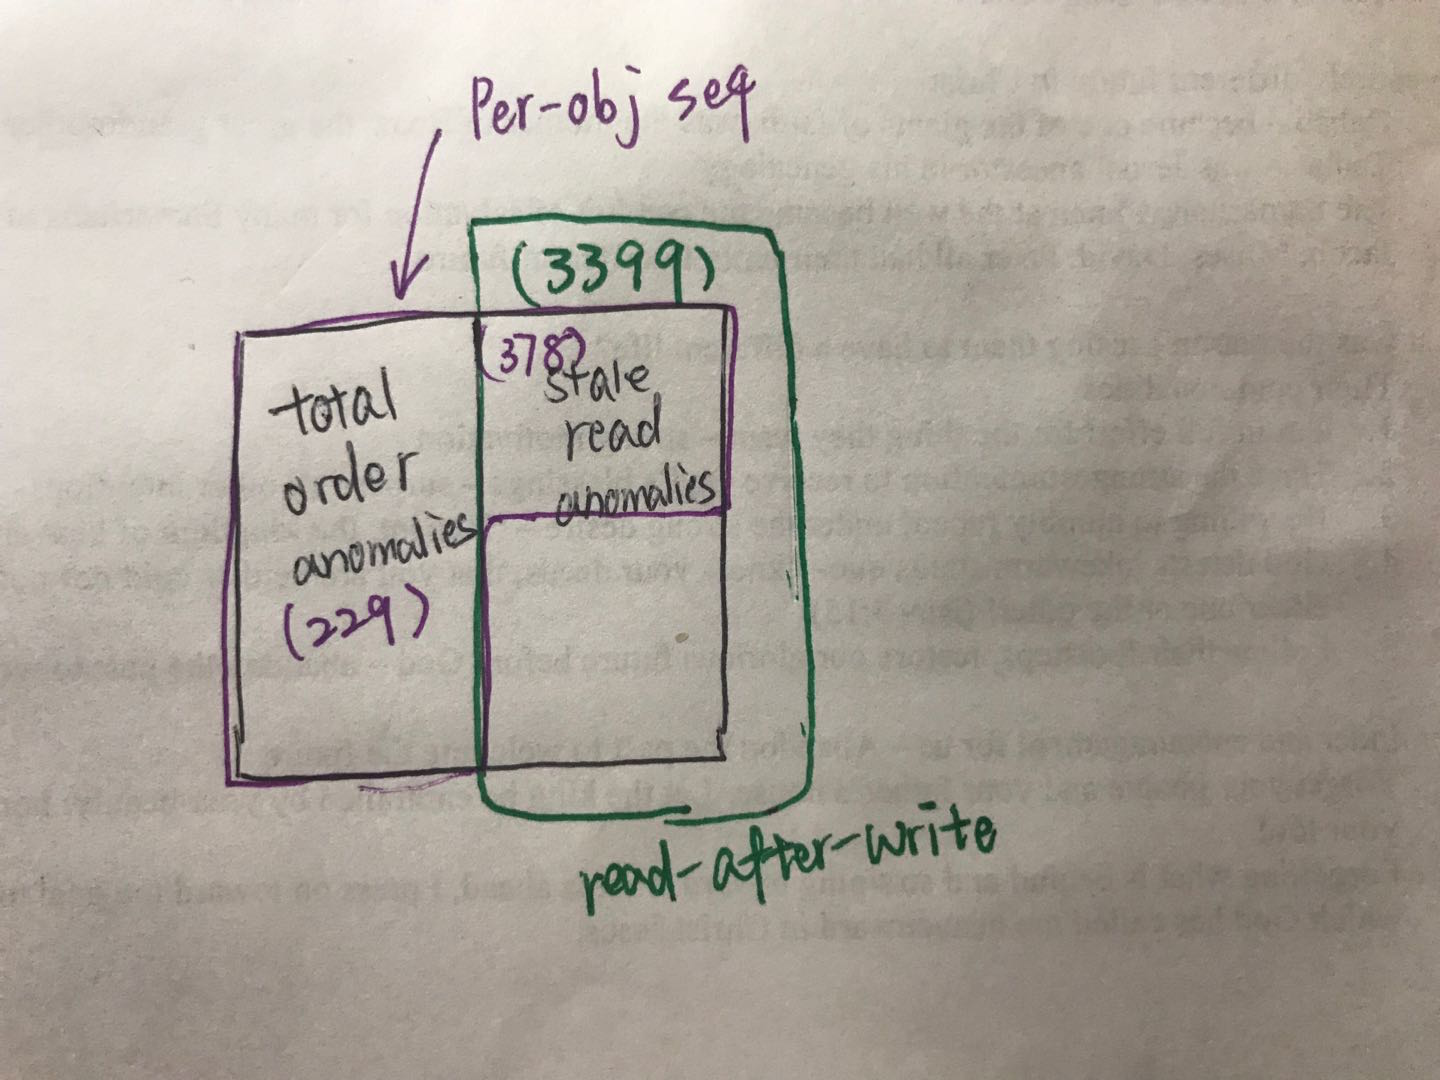
\includegraphics[width=5cm, height=4cm]{0209-02.jpeg} 
		 \caption{Illustration of statistic relationship between two consistency models}
		 \label{0209-02}
		 \end{figure}
         \end{answered}
         
   \item What performance vs consistency tradeoffs are made by Yahoo's different read types (read-any, read-critical, and read-latest)?
         \begin{answered}
    	 \texttt{Read-any} emphasizes performance over consistency.Since the latest read doesn't need to reflect the latest write (i.e.,
    	 we can still read the stale version of the record even after a sucessful write), we can maximize our performance by return a valid
    	 version of record from the records' history. However, for \texttt{Read-critical} and \texttt{Read-latest}, we emphasize the consistency
    	 over the performance. \texttt{Read-critical} requires the returned version has to be strictly newer or the same as the specified version
    	 and \texttt{Read-latest} requires the return has to be the latest copy of the record that reflects all the previous successful writes.
    	 These two types of reads require the squential consistency for the record and at the same time, if the local cahced copy becomes stale,
    	 we need to fetch a new copy from remote replica, which implies that the performance of these two APIs will be lower than \texttt{Read-any}'s. In addition, since \texttt{Read-critical} can return any version of the record as long as the requirement is met, there
    	 are a fraction of record history that satisfy the constraint and any one of them can work. However, \texttt{Read-latest} can only return
    	 the latest one. Thus, \texttt{Read-latest} has the strongest consistency among the tree with the worst performance.
         \end{answered}
\end{QandA}

\subsection{Feedback}

\subsubsection{Samantha's Comment}
Your discussion of leases is generally correct, but I don't think it's normally possible to have multiple strong leases for one object. The main idea behind strong leases is that one cache has exclusive use of the object.

You mix up stale read anomalies and total order anomalies a bit in your paragraph, but your diagram is correct. Read-after-write only has stale read anomalies.

\subsubsection{Zeyuan's Response}
I'm referencing Jim Gray's lease paper ("Leases: An Efficient Fault-Tolerant Mechanism for Distributed File Cache Consistency") and I assume the "lease" term in the paper actually means "strong lease" in our context. In the section 2 of the paper, there is one sentence "When a client writes a datum, the server must defer the request until each leaseholder has granted approval or the term of its lease has expired.", which includes the term "each leaseholder". In addition, he gives an example of a file cache using lease and he states that "When a new version of latex is installed, the write is delayed until every leaseholder has approved the write."
Those sentences make me think if any object in the cache can have multiple strong leases.

Please let me know if I misunderstood the paper.

\subsubsection{Samantha's Comment}
I think the paper is just a generalization of the leases we talked about in class. Strong leases, as we discussed them in class, grant exclusive privileges to a cache, so no coordination is required. Giving out multiple leases and requiring coordination between them is definitely a valid system, but that's a bit more complicated than how the slides described leases. That combines some of the ideas of leases and invalidations. If this all makes sense, that's awesome. I just want to make sure you're clear on the basic leases before moving onto a more nuanced view of precisely what leases do and the range of properties that they can provide.
\section{Feb 16 Review Questions}
\begin{QandA}
   \item Chain replication provides both high availability and strong consistency. What does it sacrifice in order to do this?
         \begin{answered}
		 Chain replication sacrifices partition tolerance. Partition tolerance requires system to continue functioning even if there
		 is a partition between nodes. However, chain replication cannot guarantee partition tolerance because master has to continue
		 monitoring the servers in case of failures and indicating the clients about which server is head and which server is tail.
		 In addition, there cannot be any network partition within a chain when each object is tied to a unique chain. If so, strong consistency
		 cannot guarantee when the update request sent to head and query sent to tail and there is a network partition in-between.
         \end{answered}

   \item From "Paxos Made Simple", choose a numbered property (P1, P2, P2a, etc.) and discuss why it is necessary for the Paxos protocol.
         \begin{answered}
		 P1 states that ``An acceptor must accept the first proposal that it receives." This property is neccessary for the Paxos protocol
		 because the safety requirement of the Paxos protocol is that one and only one value has to be chosen. This indicates that no matter 
		 scenario, a value has to be chosen. One possible situation is that there is only one value propsed by a single proposer. In this case,
		 the safety requirement of the Paxos protocol requires to choose a value and P1 property exactly guarantees no matter what scenarios,
		 a value will be chosen.
         \end{answered}
         
   \item Chubby combines leases and invalidations for its caching mechanisms. What benefits does it get from this combination?
         \begin{answered}
%		 The invalidations ensure that all the clients that access the data can get a consistent view of the data. When
%		 the modification of the data happens, the master sends out the invalidation requests but the modification happens only when
%		 either the client invalidates its cache or the lease on the cached data expires. Lease allows the clients to use
%		 the cache for the read when invalidation request received, which is especially useful when reads outnumber writes. 
		 The invalidation request is sent out to all the clients and then the master is waiting for the invalidation acknowledgement. If we
		 use invalidation only, the master may keep waiting until all clients respond. In this scenario, some client may be outage and fail
		 to response and the master may wait for a long time. However, with the help of the lease, the server can wait for the amount of lease
		 time and then directly update the value even some client may fail to response. This helps to improve the performance of the write.
		 In other words, lease reduces the worst scenario waiting time of the server. In addition, the cached data protected by lease can avoid indefinitely updates while the client still need to access the file. Without lease, the client may be forced to update its cached data 
		 during its access to the data, which causes uncessary read delay. In other words, lease allows the read from the cache during the time
		 when the server is waiting for all the invalidation reponse. This is especially helpful when the lease expired just when the invalidation
		 response arrives at the server.
         \end{answered}
\end{QandA}
\section{Feb 16 Review Questions}
\begin{QandA}
   \item Assuming no upper bound on message delivery time, it's impossible to completely provide the four properties of consensus (Validity, Uniform Agreement, Integrity, and Termination). Which of the properties does Paxos sacrifice, and how?
         \begin{answered}
		 Paxos sacrifices termination property. Termination states that every node will eventually decide on a value. If we assume there is no
		 upper bound on message delivery time, then it is possible that before an acceptor gets its \texttt{PREPARE} message, it receives a higher 
		 offer.Since the message delivery time can be arbitrary long, the likelihood that this scenario happens is very high. Since the proposer 
		 receives a higher offer from its acceptor and it must change its value to the higher offer from its acceptor before sending out 
		 \texttt{ACCEPT}. However, since the message delivery time can take arbitrarily long, then one of the acceptors may receive even higher offer 
		 and returns \texttt{NACK} to the proposer. So, the proposer must retry again. Thus, Paxos cannot guarantee termination with the unbounded 
		 message delivery time assumption.
         \end{answered}

   \item Paxos is often implemented using a distinguished or "leader" proposer. Why can't it assume that there is always one proposer?
         \begin{answered}
		 Paxos is a fault-tolerant distributed consensus algorithm which ensures that the clients request will not be blocked (not the same
		 as being rejected) if a majority of processes are working. If Paxos assumes that there is always one proposer, then the above guarantee
		 cannot hold as now we have a single point of failure and we need to run the leader election process which may block the requests and
		 thus hinder the availability. ``Leader"
		 proposer is used as a optimization trick in Paxos to simply message numbering and ensure no contention. It is not a necessary condition
		 for ``a majority of processes are working" required by Paxos. 
         \end{answered}
         
   \item What's the difference between ballot numbers and slot numbers in Paxos Made Moderately Complex?
         \begin{answered}
         Ballot number is the same as the proposer number mentioned previously in Paul's slide. It is used as a way to reach consensus on 
         which serial of commands to agree upon across acceptors. However, slot numbers are served as indices to a serial of commands. Specifically, commands are associated with slots and each slot is indexed by a slot number. 
         \end{answered}
\end{QandA}





\section{Mar 02 Review Questions}
\begin{QandA}
   \item What are the pros and cons of having a leader in a consensus protocol?
         \begin{answered}
		 The pros of having a leader is that the servers can reach a consensus quickly. However,
		 the cons of having a leader is that when the leader is down, we need to have a election procedure to select a leader
		 and during the election we may not able to accept the requests. Thus, having a leader in a 
		 consensus protocol may impact the availability of the system.
         \end{answered}

   \item Do you think RAFT is easier to understand than Paxos? Why or why not?
         \begin{answered}
		 Yes. I think RAFT is easier to understand. One reason is that RAFT has a leader and we
		 intuitively, that usually how we think about a consensus can reach in real life. In addition,
		 RAFT implements a heartbeat so that we can know whether a server is live or not and the how the data
		 is commited in the log is much easier to understand than Paxos.
         \end{answered}
         
   \item What benefit does Sinfonia gain by using minitransactions instead of general transactions?
         \begin{answered}
		 Minitransactions allow user to performing batch updates, which elmininates multiple network round-trips
		 that can happen to general transactions. In addition, minitransactions can be executed within the commit protocol,
		 which avoid two round-trips to commit and additional round-trips to start and execute in general transactions.
		 Lastly, minitransactions can execute in parallel with a replication scheme.
         \end{answered}
\end{QandA}





\section{Mar 23 Review Questions}
\begin{QandA}
   \item Pick an assumption from the DDS paper and explain how reasonable you think it is and how it affects the design in the paper.
         \begin{answered}
         One assumption made in the DDS paper is that the cluster does not have network partitions and the software components in the
         cluster are fail-stop. Since there is no network partition in the cluster, then any partition in the replica group can be
         used to service a \texttt{get()}, and all partitions in the replica group can be synchronously updated for \texttt{put()} or 
         \texttt{remove()} operations. With partition, we cannot have the replica group and we cannot expect any partition in the replica
         group can be used to service \texttt{get()} operation. In addition, the without any network partition assumption also helps with
         the trie implementation of the data partitioning (DP) map and support the strong consistency using 2PC protocol. Fail-stop assumption
         is required to provide consistency model using 2PC. If there is byzantine problem, replica may repond even in an error status, which may
         lead to inconsistent key-value pairs.
         \end{answered}

   \item  How does Chord's combination of fingers and successors allow it to achieve its desired correctness and performance properties?
         \begin{answered}
		 Chord requires only $O(\log N)$ lookups to find the node for a given key. Suppose we try to find the successor node of a key $k$, which
		 is the location for the key. To do so, we consult our finger table. If $k$ appears in the \texttt{start} column of the fingers table, we 
		 are done (the number in the same row under \texttt{succ.} column is the target node). If not, we figure out which \texttt{interval} covers $k$ and then we find the node's ID that is most immediately precedes $k$
		 and we ask that node to find the sucessor node of $k$ for us. Thus, we always move closer towards the precedessor of $k$, which will leads
		 us to the target node. $O(\log N)$ appears because we halve the distance between the node handling the query and the predecessor of $k$ 
		 each query step towards $k$.
         \end{answered}
\end{QandA}





\section{Mar 30 Review Questions}
\begin{QandA}
   \item How do Byzantine failures break a previous algorithm we've looked at (you pick another algorithm and compare)?
         \begin{answered}
         For example, server with Byzantine failure can make the fake vote to other servers during the leader election phase of the RAFT.
         Thus, there can be multiple leaders to send out commit request, which may lead to serious consensus problem. Another
         example is chord. Byzantine failure can make a server mistakenly states that the key is not located in it or the server
         can give wrong information in the finger table that breaks $O(\log N)$ lookup guarantee.
         \end{answered}

   \item  What assumptions does Coda make about system behavior that allow it to be effective?
         \begin{answered}
         Coda assumes that at certain times, a client may be temporarily unable to communicate with some or all
         of the servers and thus, coda uses to cache to allow users to read and write files even they are disconnected.
         In addition, Coda assumes access and sharing patterns typical of academic and research environment. In other words,
         Coda is not built for applications that need highly concurrent, fine granularity data access. This assumption
         makes Coda to adopt Optimistic Replica Control, which provides high availability by permitting reads and writes 
         everywhere. Since the concurrent access is low (i.e., the low degree of write-sharing typical of Unix), modification
         conflicts for one file by many users may be low and thus, the chance that Coda has to notify the users to resolve
         conflicts is small, which does not impact usability much. 
		 Furthermore, Coda assumes clients can communicate with the servers over a high bandwidth network. As the result, the 
		 process of reconnecting and propagting changes can be done about a minute. Also, the small amount of data makes
		 the storage requirement on clients low as well (e.g., 100MB), which helps with the fast propagation after the reconnection.
         \end{answered}
\end{QandA}





\section{April 06 Review Questions}
\begin{QandA}
   \item  What does Petal sacrifice in order to achieve its high consistency and low latency? (Hint: Look at the performance test setup.)
         \begin{answered}
		 Petal relies on the ATM hardware to achieve its high consistency and low latency. However, due to the characterstics of ATM hardware,
		 which is used for voice and video, Petal is vlunerable to network partition. If the data is large, there might be network congestion,
		 which fails the high consistency and low latency provided by Petal.
         \end{answered}

   \item  Frangipani was written about 20 years ago. How would you expect the design decisions in this system to hold up to today's needs?
         \begin{answered}
		 Frangipani uses multiple-reader/single-writer locks to coordinate the access to the virtual disk and to keep the buffer caches
		 coherent across the multiple servers. However, when compared with modern system like GFS, the lock service might be the bottleneck
		 for the system performance because it does not allow the concurrent write, which is a critical factor for modern system
		 high performance (i.e., high throughput).		 
         \end{answered}
   \item How does the Google File System's relaxed consistency model benefit the system design?
         \begin{answered}
         GFS's relaxed consistency model greatly simplfies the file system design without imposing large burden on the application.
         In addition, relaxed consistency model allows each machine forwards the data to the ``closest" machine in the network topology
         that has not received it, which avoids the network bottlenecks and high-latency links as much as possible. Furthermore, relaxed
         consistency model decouples the data flow from the control flow, which improve performance by scheduling the expensive data 
         flow based on the network topology regardless of which chunkserver is the primary. Lastly, a strict consistency model
         may bring complex implementation of the file system. However, with a few simple techniques (e.g., relying on appends rather than overwrites, checkpointing, and writing self-validating, self-identifying records) on applications, we can much reduce implementation complexity.
         \end{answered}
   \item How is BigTable able to avoid having the master be a bottleneck?
         \begin{answered}
         Client library caches tablet locations, which avoids much traffic to visit master querying the tablet locations.
         \end{answered}
\end{QandA}





\section{April 13 Review Questions}
\begin{QandA}
   \item  In Dynamo, Table 1 lists several approaches that the designers used to address their challenges and provides an advantage for each. Pick two techniques and list a disadvantage for each.
         \begin{answered}
         Consistent hashing has its own two problems: 1. random position assignment of each node on the ring leads to non-uniform data and load
         distribution; 2. the algorithm is oblivious to the heterogeneity in the performance of nodes. Dynamo tends to fix this problem by introducing
         ``virtual nodes". However, by using virtual nodes, the system complexity increases as virtual nodes need to maintain extra information
         about whether they are in the same physical node. In addition, when we add nodes into the ring, we need to assign the tokens such that
         the load can be distributed uniformly, which further increases the system complexity. Furthermore, the gossip-based membership protocol
         and failure detection adds extra burden to each individual node and it can hardly scale to more 1000 servers.
         \end{answered}

   \item  How is RAMCloud's design affected by keeping all data in DRAM?
         \begin{answered}
         RAMCloud requires all data in DRAM. Due to this requirement, RAMCloud requires all the DRAM has an auxiliary power source, which ensures
         that buffers can be written to stable storage after a power failure. In addition, since all data has to be in DRAM, during the recovery,
         all the data has to be recovered into DRAM instead of on the SSD or hard disk, which leads to the unwanted disk I/O and the recovery scheme
         complexity.
         \end{answered}
\end{QandA}





\section{April 20 Review Questions}
\begin{QandA}
   \item How does the size of a task affect MapReduce?
         \begin{answered}
         MapReduce takes a user-submitted job and maps to $M$ tasks and then reduce to $R$ tasks. As shown in the paper, the master
         must make $O(M + R)$ scheduling decisions and keeps $O(M \ast R)$ state in memory. Thus, given the job size fixed, the smaller
         the task in each phase (map phase or reduce phase), the larger the variable is ($M$ or $R$). Accordingly, the master will have
         more scheduling decisions to make and keep more state in memory. However, if the task size is too big, then the advantage of 
         parallel execution on a large cluster offered by MapReduce goes in vain.
         \end{answered}

   \item Spark uses a very different mechanism for fault tolerance than most systems we've studied so far. What's one assumption that allows Spark to use this method?
         \begin{answered}
         Spark uses a distributed memory abstraction called Resilient Distributed Datasets (RDDs), which is a read-only, partitioned collections
         of records to achieve the fault tolerance. Since RDDs are immutable, then we can effectively recompute the faulty RDDs given the initial
         RDDs and the lineage graph that is from initial RDDs to the faulty one.
         \end{answered}
   \item Describe one way in which a datacenter has different needs or limitations than a single machine or small cluster.
         \begin{answered}
         Compared to a single machine, datacenter has disadvantage in terms of both latency and bandwidth. Usually, a single machine can 
         access its DRAM in 100 ns. However, for machines on rack to access other machine's DRAM in the same rack, the latency can take
         300 $\mu$s. Similarly, machine that accesses its local DRAM has bandwidth 20 GB/s. However, for the same machine to access other
         machine's DRAM within the same rack, bandwidth drops to 100 MB/s. When compared to small cluster, datacenter has to worry about
         the enery consumption, indoor humidity, and indoor temperature. In addition, the probability of a single machine failure at any time
         can become more noticeable in a datacenter than in a small cluster.
         \end{answered}
\end{QandA}





\section{April 27 Review Questions}
\begin{QandA}
\item What's a tradeoff mentioned in Tensorflow between synchronous and asynchronous coordination?
\begin{answered}
Synchronous coordination never has stale parameter values in training steps. However, this comes with the cost of 
limited throughput. On the other hand, asynchronous coordination may have stale parameter values and additional training 
steps but we can have increased throughput. Machine learning algorithm like SGD and neural network is robust to stragglers
and thus, asynchronous coordination is considered to be the better coordination protocol.
\footnote{We can asychronously write to files because we don't care about synchronous because machine learning algorithmcan afford the cost to 
compute one more training iteration}
\end{answered}

\item How does the parameter server model reduce network usage?
\begin{answered}
Parameter server uses \texttt{push} and \texttt{pull} operations to push its entire local gradient into the servers, and
then pull the updated weights back. By updating parameters in batch, parameter server avoids the network overhead of each individual
parameter update. This updating scheme naturally fits with the batch update form of machine learning algorithms. In addition,
parameter server compresses the messages sent across the nodes, which further reduces network usage.
\end{answered}
\end{QandA}






\end{document}
